\section{Analiza złożoności i~estymacja zapotrzebowania na zasoby}
Pierwszym i~niezbędnym krokiem przy pracy na stanowisku laboratoryjnym było zapoznanie się z~dostępną architekturą sprzętową oraz wybór środowiska programistycznego. Następnie, zapoznano się i~opisano standard OpenCL, w~ramach którego implementowano algorytm rekonstrukcji obrazu na kartach graficznych. Należało bowiem poznać szczególne wymagania oraz ograniczenia wynikające z~jego użycia. Dalszą część rozdziału stanowi oszacowanie złożoności pamięciowej i~obliczeniowej wybranego algorytmu odtwarzania obrazu.
\subsection{Sprzęt uruchomieniowy}
Dostępny w~laboratorium komputer składał się z~wielordzeniowego procesora klasy Intel i5 oraz dwóch kart graficznych firmy Nvidia GeForce GTX670. W~poniższej tabeli zebrano ich główne parametry:

\begin{table}[H]
\begin{center}
\begin{tabular}{|c|c|}
\hline
         & Nvidia GeForce GTX 670  \\
\hline
        Liczba rdzeni & 1344 \\
\hline
        Częstotliwość bazowa & 915 [MHz] \\
\hline
        Pojemność pamięci & 2048 [MB] \\
\hline
        Magistrala & 256 [bit] \\
\hline
\end{tabular} 
\caption{Wybrane parametry kart graficznych Nvidia GTX 670}
\label{tab:PGU}
\end{center}
\end{table}

Liczba rdzeni wykorzystywanej przez nas karty graficznej jest wprost imponująca. Potencjalnie, wykorzystanie tej ilości jednostek obliczeniowych może dać kolosalne korzyści czasowe. Program, który w~skuteczny sposób wykorzystuje powyższe zasoby, musi dokonać kilku niskopoziomowych optymalizacji. Doskonałą lekturę w~tym zakresie stanowiła książka opisująca bibliotekę OpenCL \cite{Scarpino2012}. Po pierwsze, należy minimalizować liczbę rozgałęzień algorytmu. Po drugie, zadania na karcie graficznej należy dzielić tak, by zależności między wątkami były jak najmniejsze - konieczność synchronizacji znacznie zmniejsza wydajność programu. Po trzecie, należy minimalizować liczbę odwołań wątków karty graficznej do pamięci globalnej - podręczne zasoby lokalne charakteryzują się znacznie mniejszym opóźnieniem. W~końcu, należy liczyć się z~każdorazowym opóźnieniem obliczeń na GPU, ze względu na dwukrotny transfer danych między hostem a~urządzeniem.

Zdecydowano się na implementację programu w~języku C++, z~wykorzystaniem środowiska Visual Studio. Wynikało to z~kilku przyczyn. Po pierwsze, wybór był konsekwencją doświadczenia zawodowego autora. Pisanie kodu w~znanym sobie języku i~środowisku znacznie przyspieszyło pracę. Po drugie, przygotowany SDK kamery Jai zawierał binding w~tym właśnie języku, co znacznie uprościło integrację tego modułu programu. C++ pozwolił twórcom z~jednej strony zdekomponować problem obiektowo, a~z~drugiej - skompilować program natywnie, licząc na optymalną wydajność. Z~perspektywy czasu trzeba jednak rozważyć, czy nie lepiej wykorzystać Pythona, z~uwagi na duże wsparcie biblioteczne tego języka, a~także czytelność i~zwartość kodu. Ostatecznym celem programu było bowiem maksymalne wykorzystanie karty graficznej, z~minimalną ingerencją komputera-hosta. Ponadto, krytyczne dla wydajności procedury można by zawrzeć w~formie skompilowanej biblioteki języka C.~Ciekawym byłoby zatem porównać nakład pracy przygotowanych programów i~ich wydajność.

\subsection{Standard OpenCL}
Jednym z~głównym wyzwań projektu było zaznajomienie się i~wykorzystanie standardu OpenCL \cite{OpenCL} do programowania w~heterogenicznym środowisku obliczeniowym. W~przeciwieństwie do rozwijanego przez firmę Nvidia standardu CUDA, OpenCL może być wykorzystywany na różnych platformach sprzętowych, o~ile tylko standard jest wspierany przez producenta. Choć OpenCL definiowuje tylko interfejs programistyczny w~języku C oraz wrapper w~C++, dostępne są również jego realizacje w~Javie, Pythonie i~innych. W~chwili pisania raportu, opublikowano wersję 2.0 tego dokumentu. Niestety, żaden z~producentów kart graficznych jeszcze go nie wspiera. Posługiwano się więc interfejsem programistycznym standardu w~wersji 1.2.

Na podstawowe pojęcia w~OpenCL składają się: \textit{host} i~\textit{device}, na których wykonywana jest aplikacja. \textit{Host} to zwykle CPU, wysyłające rozkazy do GPU (\textit{device}), w~szczególności w~celu wykonywania \textit{kerneli}, czyli dynamicznie kompilowanych programów. Pojedynczy rdzeń procesora karty graficznej zwany jest \textit{work-itemem}. Pewien zbiór tychże stanowi \textit{work-group}. Jednostki obliczeniowe rozróżniane są globalnym identyfikatorem \textit{globalID}, a~grupy - \textit{localID}. 
Pamięć \textit{device} możemy podzielić na 4 typy: private, local, constant, global. Ich dostęp możliwy jest odpowiednio: \textit{work-item}, \textit{work-group} oraz cały \textit{device}. Cechują się one kolejno rosnącą pojemnością. Niestety, wielkość pamięci idzie w~parze z~coraz dłuższym czasem dostępu.

\subsection{Wykorzystanie biblioteki ViennaCL w~projekcie}
Pokrótce analizując kod źródłowy pakietu $\ell_1$-MAGIC, szybko zrozumiano, że napisanie i~przetestowanie \textit{kerneli} dla karty graficznej będzie zadaniem karkołomnym. Standard w~swej naturze jest bardzo niskopoziomowy, co z~jednej strony zapewnia elastyczność - ale z~drugiej, niską efektywność pracy. Zdolność do debugowania kodu przeznaczonego na kartę graficzną jest ograniczona. W~dodatku, współbieżna praca wielu wątków programu jest częstym błędem występowania trudnych w~zreprodukowaniu i~zrozumieniu błędów. Przygotowanie efektywnych solverów układów liniowych nie jest zadaniem trywialnym. Z~tego powodu zdecydowano się wykorzystać bibliotekę \textbf{ViennaCL} \cite{ViennaCL}, która oferuje wysokopoziomowy interfejs programistyczny do przygotowania i~uruchamiania zadań na karcie graficznej, zawiera wiele przydatnych, gotowych funkcji, takich jak solvery układów liniowych, metody dekompozycji macierzy, a~w~końcu - jest niezwykle elastyczna, pozwalając na uruchamianie własnoręcznie napisanych \textit{kerneli}.

\subsection{Oszacowanie złożoności algorytmu TVQC}
Dokładna ocena złożoności czasowej i~pamięciowej algorytmu TVQC wydaje się być trudna. Tym niemniej, wnioski płynące z~krótkiej analizy problemu wydają się oczywiste. Najbardziej kosztownym czasowo i~obliczeniowo krokiem algorytmu jest rozwiązanie formy kwadratowej. Rozważania ze wstępu tłumaczą konieczność wykorzystania iteracyjnej metody rozwiązywania tego układu. W~swym doskonałym artykule, autor biblioteki \textit{ViennaCL} porównał teoretyczną i~praktyczną wydajność architektur CPU i~GPU.~Poza specyficznymi wyjątkami (operacje mnożenia dwóch gęstych macierzy), wydajność kart graficznych zależy w~głównej mierze od przepustowości magistrali pamięci. Uzyskane od autora artykułu informacje wskazują, że mnożenie rzadkich macierzy na GPU osiąga praktyczną wydajność ok. $1\%$ piku teoretycznego. Obliczenia arytmetyczne uzyskiwane na karcie graficznej są więc "za darmo" - karta głównie czeka na dane. Okazuje się jednak, że wysokiej klasy karty graficzne osiągają w~praktycznej implementacji metody gradientu sprzężonego lepsze rezultaty dla problemów dużych rozmiarów, z~uwagi na większą przepustowość pamięci, która w~pewnym momencie kompensuje konieczność kopiowania danych \textit{host-device}. Najlepiej ilustrują to pomiary wydajności metody gradientu sprzężonego, wykonane przez twórców ViennaCL i~przedstawione na rysunku ~\ref{fig:CGPerformance}.
\begin{figure}[H]
\centering
	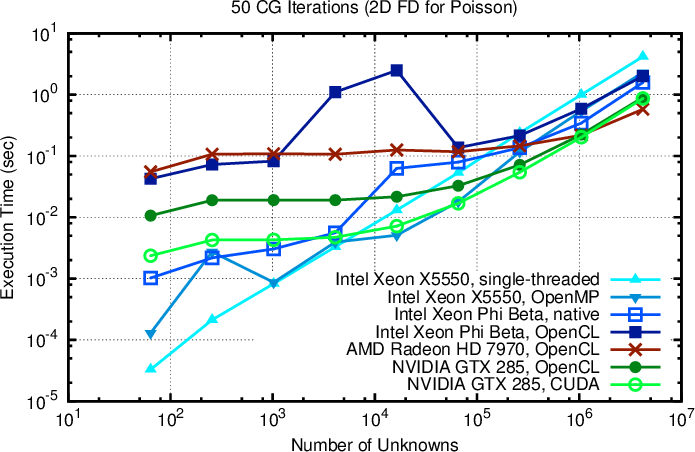
\includegraphics[width=0.8\textwidth]{rysunki/cg-timings.png}
\caption{Porównanie wydajności algorytmu CG dla wybranych platform sprzętowych \cite{ViennaCL}}
\label{fig:CGPerformance}
\end{figure}

Wnioski płynące z~analizy złożoności TVQC są następujące: kluczowy wydaje się taki podział prac między CPU a~GPU, by karta graficzna wykonywała tylko operacje w~dużej skali. Ponadto, należy zadbać o~jak najlepsze wykorzystanie przepustowości pamięci karty graficznej, np. poprzez dostęp do niej w~sposób "coalesced" \cite{CoalescedIntro}, tzn. by work-item'y w~obrębie work-group'y żądały jednoczesnego dostępu do pamięci globalnej.